\documentclass[10pt,letter]{article}

\usepackage{graphicx}
\graphicspath{ {Figures/} }
\usepackage{tikz}
\usetikzlibrary{shapes,arrows}
\usepackage{amsmath}
\usepackage{amsfonts}

\DeclareMathOperator*{\argmax}{argmax}
\DeclareMathOperator*{\argmin}{argmin}

\begin{document}

\section*{Title}
Soft material deposition geometry detection using laser triangulation machine vision

\section*{Authors}
van Houtum, Gijs Johannes Jozef \\ 
\texttt{gjjvanhoutum@uwaterloo.ca} \\
\\
Vlasea, Mihaela Luminita\\
\texttt{mihaela.vlasea@uwaterloo.ca} \\
\\
Multi-Scale Additive Manufacturing Laboratory \\
Department of Mechanical and Mechatronics Engineering \\
University of Waterloo \\
Waterloo, Canada 

\section*{Keywords}
Additive Manufacturing, Material extrusion, Material jetting, 3D printing, Laser Triangulation, Machine Vision, Structured Light, Feedback Control, Thresholding 

\section*{Abstract}
Conventional manufacturing processes lack the free form capabilities additive manufacturing has. Achieving accuracy and short production time are however challenging to achieve. If these problems could be resolved, it could replace conventional methods and mass produce more complex parts.

Feedback control of the deposited material geometry in soft material extrusion processes could improve the accuracy of parts. Feedback of geometry is possible through the implementation of a triangulation based vision system. Image processing algorithms exist to extract geometric features such as height and width but lack robustness against noise and automation since many tuning parameters are needed for operation. 
 
This research proposes a new image processing algorithm able to detect height and width of soft material additive manufacturing processes. The algorithm is developed to operate under pixel saturation and laser line induced noise. Automation is improved since only a single initial parameter is needed for operation.
The methods used for the algorithm are tested by comparison against commonly used methods such as Otsu's thresholding and general differencing methods.

\textbf{What numerical data and results should be added?}


\section{Introduction}

Additive Manufacturing (AM) has the ability to produce more complex products than conventional manufacturing processes \cite{stucker2010additive}. Dimensional accuracy, repeatability and short production time are however challenging to achieve within AM processes. Specifically, extrusion based additive manufacturing processes for soft materials \cite{liravi2017additive}. If the prescribed problems could be overcome AM could replace these conventional methods for mass production and leverage the free form capabilities. 

Soft material based processes are typically divided into material jetting and material extrusion \cite{calignano2017overview}. The former uses drop-on-demand technology where the nozzle dispenses droplets of material, layer by layer. The latter is referring to the process where the material is extruded onto the build platform. 

Control of deposition geometry is often achieved in open-loop. No geometric measurement of the deposition is used as feedback during the printing process. Alternatively, experimental static parameter calibration is conducted to tune the system for nominal operation \cite{magnoni2017robotic}. The dynamics of the system are however neglected and problems such as over- and under-filling at off-nominal system states compromise accuracy.

The implementation of a real-time deposition geometry feedback controller could improve dimensional accuracy. Vision-based feedback control of deposition extrusion rate as described in \cite{hoelzle2008iterative} showed improved accuracy. The controlled variable does however not control the deposition geometry directly. Recent work \cite{faes2016process} describes the application of a laser-camera triangulation based vision (LT) system to monitor the geometry of soft material processes after deposition. Work on the usage of a LT system for direct geometry control is however limited. 

\subsection{Workflow of Vision-based Detection}
Image processing algorithms used for geometry detection from images generated by a LT system can be divided into image segmentation, laser line extraction and feature extraction as proposed in \cite{li2007recent}.

\subsubsection{Image segmentation}
The goal of image segmentation is to divide the image into separate sections to find important regions-of-interest (ROI) and improve computational efficiency. 

Manual selection of region size and position as described in \cite{huang2012development} is only effective for detection of static positioned objects. Another paper \cite{wang2014weld} manually selects ROI size while position is determined by the peak average column intensity of the image in gray-scale. This allows for deposition movement with constant region size. An algorithm to find the ROI position in both directions and determine the size automatically is described in \cite{xu2004features} where manual thresholding is used to separate fore- and background. The region is determined by forming a bounding box around the remaining pixels. 

Laser line segmentation is often achieved through thresholding methods. Global thresholding is used in \cite{zhang2007vision} where the thresholding value is determined by inspection of the image histogram. In \cite{wang2014weld} the threshold value is automatically determined by using the average of the maximum and minimum pixel intensity. A commonly used histogram thresholding method based upon maximizing the variance between the fore- and background is Otsu's method \cite{otsu1979threshold}. 

\subsubsection{Laser line extraction}
Line extraction is used to convert the laser line segment to a pixel position vector representing deposition geometry. 

A common method \cite{huang2012development} \cite{nguyen2014laser} \cite{kim1995robust} \cite{li2010measurement} is to define the laser line position at every column or row as the pixel position with the highest intensity in the gray-scale image. Others \cite{davis2011vision} \cite{xu2004features} \cite{zhang2007vision} take the maximum pixel difference of the segment edges and set the middle as the laser position. There also exist methods based upon morphology and the watershed algorithm as described in \cite{li2007recent}.

Noise makes it often impossible to detect the laser position for a column or row accurately and filtering methods are often used to reduce noise. Interpolation with a moving average filter \cite{wang2014weld} can be used to account for inhomogeneities in the laser line. The distinction between the laser line and background regions is often disturbed. Convolution based filtering \cite{huang2012development} with different kernel sizes and shapes are used to smooth the image. In \cite{zhang2007vision} a median filter is used where each pixel value is replaced by the median of neighboring pixels. There are also frequency based filtering methods as applied in \cite{uzun2005fpga} and wavelet methods such as in \cite{liu2006image}. Removing noise by taking the smallest intensity of each pixel from consecutive images is described in \cite{li2010measurement}.

\subsubsection{Feature Extraction}
Extraction of geometric features is application specific. A common approach is to label certain point on the laser line as feature points. Dimensions can then be calculated by the difference between those points. The simplest methods \cite{li2010measurement} \cite{huang2012development} rely on taking second derivatives of the laser line and labeling the absolute values as feature points. In \cite{kim1995robust} the laser line is segmented into small sections connected to each other (feature points) using polygonal fitting. Paper \cite{davis2011vision} decides if a point is a feature point based upon linguistic rules set by a threshold. 

\subsection{Challenges within Vision-based Detection}

\subsubsection{Hardware induced challenges}
A typical image generated by the TL system is shown in Figure \ref{fig: data_problem} where the laser is positioned at the bottom of the image. Around the laser line are scattered reflections visible. A perfect laser should focus all light to a single line. The laser module is the source of these unwanted reflections and lens distortion or contamination could be the source of these artifacts. Since the TL system operates in environments with heat and soft material it is possible that the lens gets contaminated. The algorithm should therefore be robust against these kinds of noise. histogram thresholding not realistic. 
\begin{figure}[!h]
	\centering
	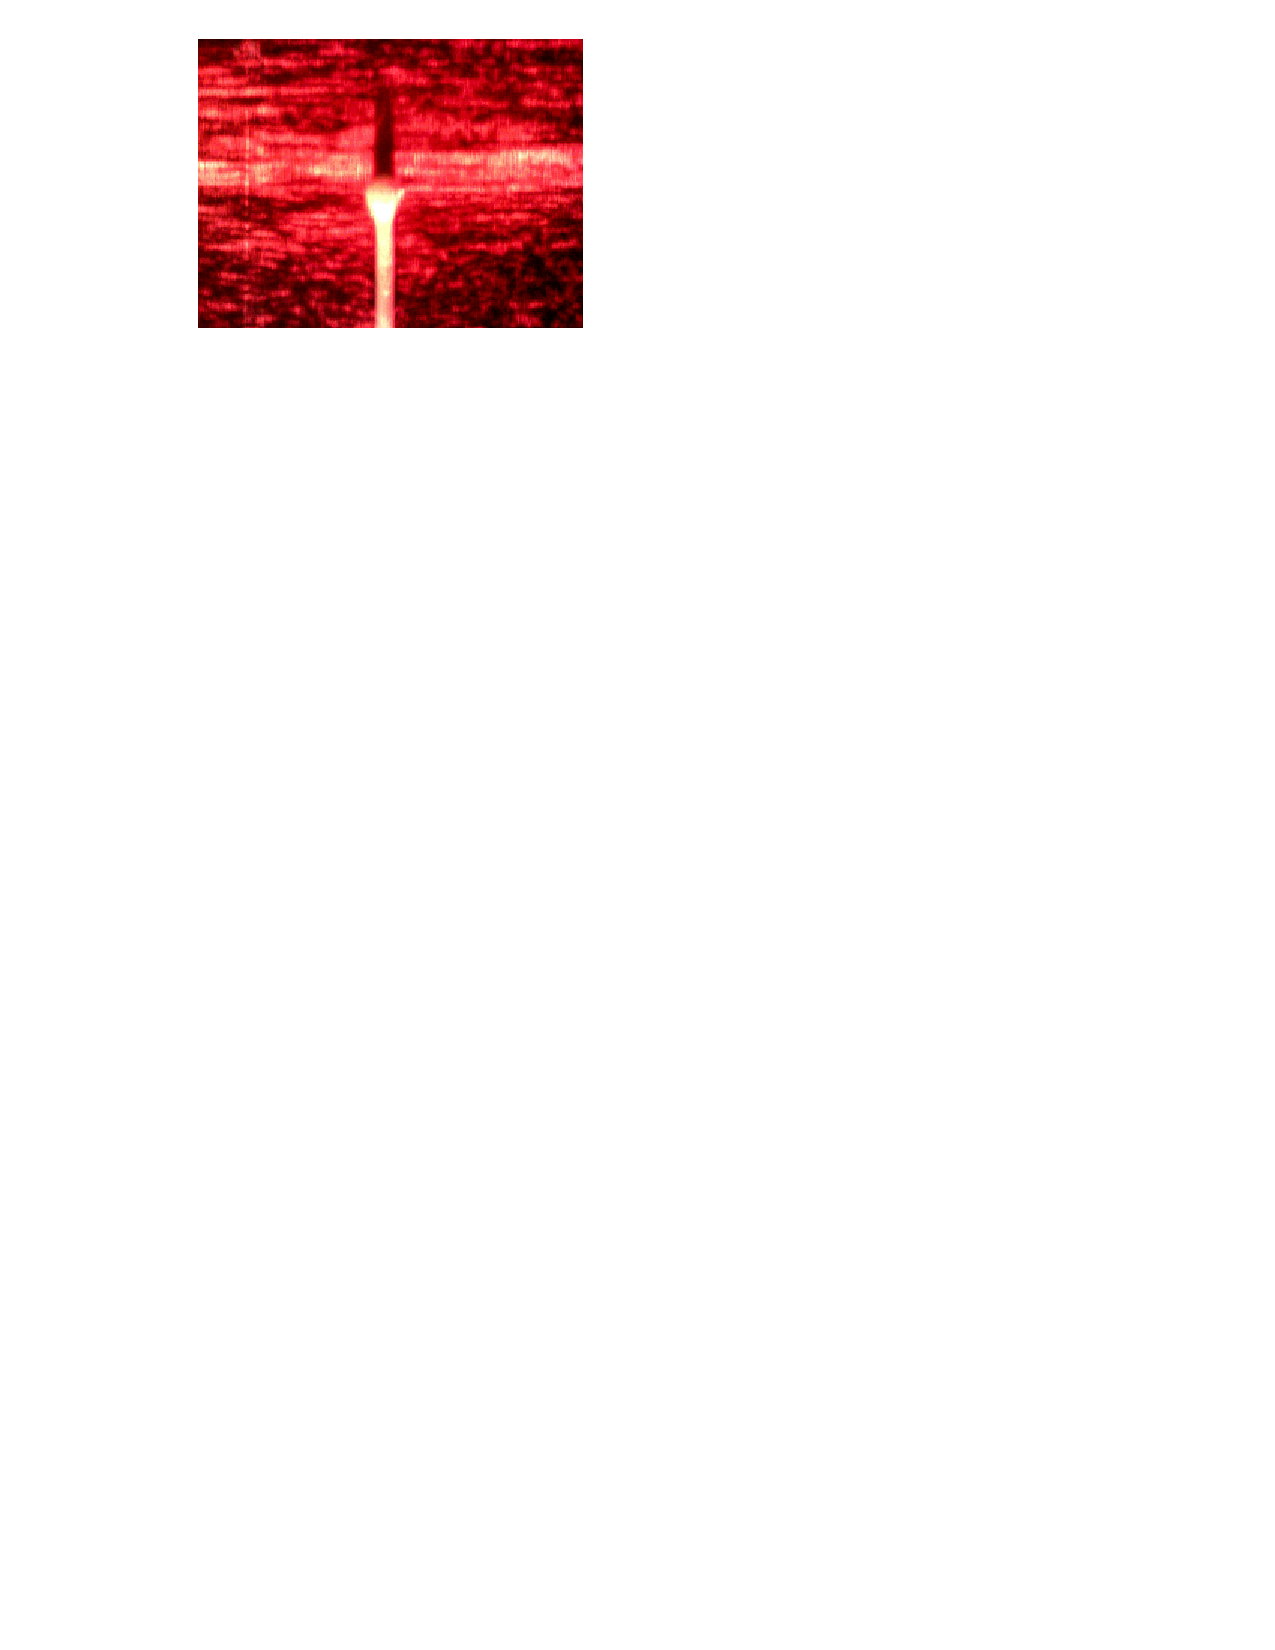
\includegraphics[width=0.6\linewidth]{data.pdf} 
	\setlength{\unitlength}{0.1\linewidth}
	\footnotesize\put(0.8,2.75){Laser Lens}
	\footnotesize\put(0.8,2.5){Induced}
	\footnotesize\put(0.8,2.25){Reflections}
   	\footnotesize\put(-8,2.3){Laser Line}
	\footnotesize\put(-8,1){Saturation}
   	\footnotesize\put(-8,3.05){Inclusion}
   	\footnotesize\put(-8,1.65){Inhomogeneity}
	\thicklines
	{\color{green}\put(0.6,2.55){\vector(-1,2){0.5}}
	\color{green}\put(0.6,2.55){\vector(-1,-2){0.5}}
	\color{green}\put(-6.6,1.1){\vector(4,1){3.3}}
	\color{green}\put(-6.2,1.7){\vector(2,1){1.5}}
	\color{green}\put(-6.8,3.1){\vector(1,0){3.5}}
	\color{green}\put(-6.6,2.35){\vector(1,0){0.5}}}
\caption{Image from TL system showing hardware induced challenges.}
\label{fig: data_problem}
\end{figure}

The print bed is a relatively flat surface and the angle of incidence of the laser light is considered equal across the bed. Deposition geometry changes and the angle of incidence differs. As a result light reflected from the deposition is hard to separate in laser line and lens artifacts. Furthermore, the width of the laser line on the bed can differ from the line on the deposition. A steep angle in the deposition condenses the laser beam to a smaller amount of pixels such that it appears smaller on the image. 

Saturated pixels are visible on top of the deposition in the image. Another material might however reflect in a different way. Changing hardware according to the use of different materials is not realistic and the problem should therefore be handled in the detection algorithm. 

\subsubsection{Algorithmic challenges}
Although ROI image reduction improves computation time, possibly important information such as laser line position outside of the ROI is lost. Inhomogeneity of the laser line could have a bad influence on the accuracy of the detection algorithm when a to small ROI is used. Region selection often involves parameter tuning such as threshold value or choosing position which leads to reduced flexibility due to the reflective properties of different deposition materials. 

Thresholding methods for segmentation are often focused at maximizing the difference between image background and laser light. Noise in the form of light reflections far from the actual laser line are equally influential for threshold determination as light from the actual laser line. Laser lens induced reflections could badly influence the performance of the thresholding methods which take all pixels into account. Pixels close to the laser line should be leading for segmentation of the laser line. 

Single channel gray-scale images are often used for image processing while multi-channel images are available. Reducing a multi-channel image to a single gray-scale intensity channel leads to information loss. Use of the full image could lead to better measurement accuracy.

Differencing methods are often used to detect edges or determine peaks. The signal-to-noise ratio is often to low to detect peaks and filtering techniques are required to extract information. Filtering has a smoothing effect which reduces noise but also affects the real signal compromising accuracy. Furthermore, tuning of cut-off frequencies introduce additional tuning parameters. 

Peak detection of intensity values across a row or column is also not possible due to the possibility of saturated pixels in the image. Edge detection should focus only on a single edge since the width of the laser line on the deposition could be compromised due to the angle of incidence of the laser light onto the deposition.

Many of the above algorithms depend on parameters which need to be tuned specifically for each application. This makes the algorithm less flexible and highly dependable on the expertise of the operator to tune the algorithm. 

\subsection{Research Motivation}

To address the challenges this research proposes a new flexible and robust vision-based detection algorithm able to detect deposition height and width for SME processes. 

In this work robustness is defined as the ability to operate under pixel saturation and reflections due to lens artifacts or contamination. An alternative method to differencing is used which is able to detect change without the need for filtering. It introduces less noise and does not rely on tuning parameters. 

A new thresholding method is introduced for segmentation which reduces the influence of scattered reflections and does not depend on parameters. Laser line edge detection is used to account for pixel saturation as well as the changing angle of incidence of laser light on the deposition.

Flexibility is defined as the ability to operate without the need for adaption. Tuning of constant parameters is therefore reduced to a minimum. Information loss is reduced through smart usage of ROI and template matching of all available channels within the image instead of single channel gray-scale.   

\section{Materials and Methods}

An overview of the vision system used for experimental data acquisition in this research is shown in Figure \ref{fig:setup_real}. The system consists out of a camera (DinoLite AM7515MZTL Edge) and a line laser (Infiniter VLM-650-30), which are fixed in position, at a relative angle to each other, by a mount bracket which is attached to a custom build soft material extrusion AM machine. The camera is connected to a laptop where custom software executes the image processing algorithm. A frame-rate of ten frames-per-second is used at a resolution of five mega-pixels (2592x1944). Optical magnification is 140x and image output is in three-channel RGB format with an eight-bit pixel depth. The line laser has an output power of five milliwatt and a wavelength of 650 [nm].
The laser is positioned at a 20 degree angle relative to the print bed. The camera is placed perpendicular to the bed and the distance between the bed and the camera glass is 19.3 [mm]. Deposition geometry is exposed to the camera through the relative angle between the camera and the laser forming a triangulation setup.

\begin{figure}[!ht]
   \centering
   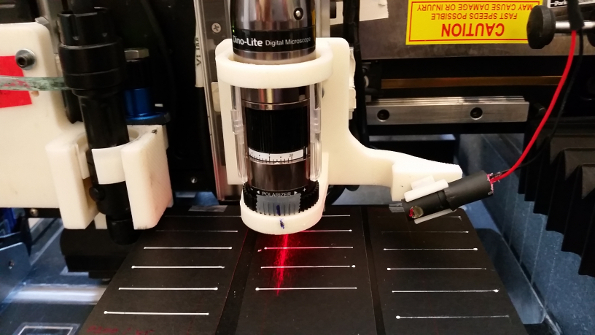
\includegraphics[width=0.6\linewidth]{setup_real.jpg}
   \setlength{\unitlength}{0.1\linewidth}
   \footnotesize\put(-8,3){Camera}
   \footnotesize\put(-8,2){UV light}
   \footnotesize\put(-8,1.75){source}   
   \footnotesize\put(-8,0.55){Laser line}   
   \footnotesize\put(1,3){Mount}   
   \footnotesize\put(1,2){Laser}
   \footnotesize\put(1,1){Deposited}
   \footnotesize\put(1,0.75){material}      
   \thicklines
   {\color{green}\put(-7,3.05){\vector(3,-1){3.4}}
   \color{green}\put(-6.9,2){\vector(3,-1){1.6}}
   \color{green}\put(-6.8,0.6){\vector(1,0){3.5}}
   \color{green}\put(0.8,3.05){\vector(-3,-1){3.1}}
   \color{green}\put(0.8,2.05){\vector(-3,-1){1.65}}
   \color{green}\put(0.8,1.05){\vector(-3,-1){1.75}}}
   \caption{Experimental vision system used for data acquisition}
   \label{fig:setup_real}
\end{figure}

For this work deposition lines are printed and UV-cured as described in \cite{vlasea2013experimental}. The syringe nozzle diameter used is 0.25 [mm] and the distance between the nozzle and the bed is 0.25 [mm]. The pressure used for deposition is 300 [kPa]. The lines are printed at 6 [mm/s] and scanned at 0.5 [mm/s] by the vision system after deposition. 

\textbf{More info needed??}

\section{Theory}
The images generated by the vision system $I \in \mathbb{Z}^{RxCxL}$ are defined as a matrix with $R$ rows, $C$ columns and $L$ layers or channels. Pixel values are accessed by subscripts $r,c,l$ and lie within the set $S_P = \{ I_{rcl} \in  \mathbb{Z} \mid 0 \leq I_{rcl} \leq 255 \}$. The set of all rows, columns and layers are respectively $S_R = \{ r \in  \mathbb{N} \mid r \leq R \}$, $S_C = \{ c \in  \mathbb{N} \mid c \leq C \}$ and $S_L = \{ l \in  \mathbb{N} \mid l \leq L \}$.

\subsection{Deposition Segmentation} \label{ssc: depseg}
The deposition is segmented from the bed such that the edge of the laser line on the bed can be attained.
Template matching and a triangle based algorithm are used to improve robustness. This step is needed such that the deposition does not influence the measurement of the laser line on the bed.

\subsubsection{Template matching}
% template matching
Template matching is used to detect deposition position. Segmenting the deposition from the bed is only possible if the bed is visible in the image. The sides of the image therefore have to belong to the bed and can be used as a template. 

The mean of $\delta^{left}_{ini}$ columns from the left and $C-\delta^{right}_{ini}$ columns from the right side of the image $I$ are used as a template for each channel to reduce influence of noise. The choice of the amount of columns used for the template is the only parameter needed for the operation of the algorithm. The templates are defined as:
\begin{equation}
T_{rl} = \frac{1}{\delta^{left}_{ini}+C-\delta^{right}_{ini}}  \sum_{c \in S_0}  I_{rcl}, \quad \forall \, (r,l) \in S_R \times S_L
\end{equation}
where $S_0 = \{c \in S_C \mid c \leq \delta^{left}_{ini} \lor \delta^{right}_{ini} \leq c \}$ 
and the sum-of-squared error for every column and layer is defined as:
\begin{equation}
SSE_{cl} = \sum^{R}_{r=1} \left( I_{rcl} - T_{rl} \right)^2 \quad \forall \, (r,c,l) \in S_R \times S_C \times S_L
\end{equation}

\subsubsection{Normalization}
Before combining the errors of each layer into a total error they are normalized. The rational behind this is that not the total error at each column is important but the error relative to the errors of columns used for the template. Therefore each error normalized where
\begin{equation}
M^{SSE}_l = \frac{1}{\delta^{left}_{ini}+C-\delta^{right}_{ini}} \sum_{c \in S_0}  SSE_{cl}, \quad \forall \, l \in S_L
\end{equation}
is the sample mean error of the columns used for each template. The sample standard deviation is defined as:
\begin{equation}
S^{SSE}_l = \sqrt{\frac{\sum_{c \in S_0} ( SSE_{cl} - M^{SSE}_l )^2}{C-1}}, \quad \forall \, l \in S_L
\end{equation}
The normalized versions then become:
\begin{equation}
NSSE_{cl} = \frac{SSE_{cl}-M^{SSE}_l}{S^{SSE}_l} \quad \forall \, (c,l) \in S_C \times S_L
\end{equation}
and the combined error is calculated as the euclidean distance between the layers as:
\begin{equation}
TE_{c} = \sqrt{ \sum_{l \in S_L} NSSE_{cl}^2} \quad \forall \, c \in S_C
\end{equation}

\subsubsection{Segmentation}
The total error curve $TE_c$ is used to separate the deposition from the print bed. The Triangle algorithm as described in \cite{zack1977automatic} is normally used as a global thresholding method and applied to image histograms. This method is however adapted to serve as a better alternative to separation based on differencing since it introduces less noise and does not need additional filtering. The first step is to form the piecewise triangle function $PT_c$ as follows:
\begin{equation}
PT_c = \left.
  \begin{cases}
    \frac{\max ( TE_c )}{\argmax_c (TE_c)} c,  & \forall \, c \in S_1\\
    \frac{\max ( TE_c )}{C-\argmax_c (TE_c)} (C - c),  & \forall \, c \in S_2\\
  \end{cases}
  \right.
\end{equation}
where $S_1 = \{c \in S_C \mid  c \leq \argmax_c (TE_c) \}$, $S_2 = \{c \in S_C \mid \argmax_c (TE_c) \leq c\}$. The deposition separation points $\delta^{left}_{dsp}$ and $\delta^{right}_{dsp}$ are defined as: 
\begin{align}
\delta^{left}_{dsp} &= \argmin_c (TE_c - PT_c), \quad \forall\, c \in S_1  \\
\delta^{right}_{dsp} &=  \argmin_c (TE_c - PT_c), \quad \forall\, c \in S_2  
\end{align}

\subsection{Laser Line Edge Segmentation} \label{ssc: edgeseg}
After deposition segmentation the laser line edge is segmented from the bed. The edge is used to account for problems due to changing angles of incidence on the deposition and pixel saturation. It serves as a reference point for height measurement. Furthermore, the width of the deposition is determinant at the position of the edge segment. 

The laser line on the print bed is separated through the application of a new thresholding method based upon the Triangle algorithm. The algorithm clarifies the edge at the point of segmentation such that reflections due to lens artifacts or distortion have reduced influence. The edge is used instead of the whole laser line since the width of the laser line could vary due to the changing angle of incidence on the deposition.

\subsubsection{Triangle Thresholding}
The image in gray-scale is used instead of all layers based upon the assumption that the laser line brightness is higher in the center and lower the further away from the middle. The image in gray-scale is $I^{gray}_{rc} = 0.299 I_{rc1} + 0.587 I_{rc2} + 0.114 I_{rc3}, \quad \forall \, (r,c) \in S_R \times S_C$. 

Using the Triangle algorithm to determine the segment where the edge is positioned is possible but unreliable due to the amount of reflections. Thresholding is therefore used to separate background from foreground before application of the Triangle algorithm. 

The optimal threshold value $t^{opt}$ is defined as the value which maximizes the distance between the maximum value of the row mean and the value at the position determent by the Triangle algorithm as the edge. The optimal threshold is:
\begin{equation}
t^{opt} = \argmin_t J_t, \quad \forall \, t \in S_P
\end{equation}
where $J_t$ is the cost function given by:
\begin{equation}
J_t = \min_r (M_{rt} - PT_{rt}), \quad \forall \, r \in S_3
\end{equation}
with $S_3 = \{ r \in S_R \mid r \leq \argmax_r (M_{rt})  \}$ and the piecewise triangle function $PT_{rt}$ at threshold $t$. The mean row intensity $M_{rt}$ is given by:
\begin{equation}
M_{rt} =  \frac{1}{\delta^{left}_{dsp} + C - \delta^{right}_{dsp}}  \sum_{c \in S_4}  I^{gray}_{rc}, \quad \forall \, (r,I^{gray}_{rc},t) \in S_R \times S_5 \times S_P
\end{equation}
where $S_4 = \{c \in S_C \mid c \leq \delta^{left}_{dsp} \lor \delta^{right}_{dsp} \leq c \}$ and $S_5 = \{ I^{gray}_{rc} \in S_P \mid I^{gray}_{rc} \geq t \}$.  

\subsubsection{Edge Segmentation}
The segment including the upper laser line edge is defined as $\delta^{lower}_{esp} < r < \delta^{upper}_{esp}$ where $\delta^{upper}_{esp}$ and $\delta^{lower}_{esp}$ are the upper and lower edge segmentation points. They are defined as:
\begin{align}
\delta^{lower}_{esp} &= \argmin_r ( M_{rt^{opt}} - PT_{rt^{opt}} ), \quad \forall \, r \in S_3 \\
\delta^{upper}_{esp} &= \argmax_r ( M_{rt^{opt}} ), \quad \forall \, r \in S_R
\end{align}
These rows are used for width extraction. If there was a clear distinction between laser line and background they would converge. The row on the bed at which the actual edge is positioned is defined as:
\begin{equation}
\delta^{edge}_{bed} = \{r \mid M_{rt^{opt}} =( M_{\delta^{upper}_{esp}t^{opt}} - M_{\delta^{lower}_{esp}t^{opt}}) / 2 \}
\end{equation}
The mean pixel value lies exactly in the middle of the mean pixel values of the rows $\delta^{upper}_{esp}$ and $\delta^{lower}_{esp}$. This method could however be improved to achieve sub-pixel accuracy.

\subsection{Feature Extraction}
\subsubsection{Width Measurement}
Deposition width is detected by the same method as used for deposition segmentation as described in Subsection \ref{ssc: depseg} . The rows containing the laser line edge, $\delta^{lower}_{esp} \leq r \leq \delta^{upper}_{esp}$, are used to determine the width of the deposition at the edge instead of the whole image. The width $W$ of the deposition at the edge segment is defined as:
\begin{equation}
W = \delta^{left}_{width}-\delta^{right}_{width}
\end{equation}
where $\delta^{left}_{width}$ and $\delta^{right}_{width}$ are the left and right column positions determent by the Triangle algorithm. They represent the deposition edges of the laser line edge segment. 

\subsubsection{Height Measurement}
The laser line on top of the deposition is segmented from the background by the same method as used for edge segmentation on the bed as described in Subsection \ref{ssc: edgeseg}. The height $H$ is defined as the difference in number of pixels between the edge of the laser line on the bed $\delta^{edge}_{bed}$ and the edge on the deposition $\delta^{edge}_{dep}$. It is given by: 
\begin{equation}
H = \delta^{edge}_{bed}-\delta^{edge}_{dep}
\end{equation}

\section{Results}
The result of template matching applied to one of the channels generated by the LT system is shown in Figure \ref{fig: template_matching}. The initial amount of columns used for the template is $130$ which is approximately $10\%$ of the image width. 

Normalization results for another image are shown in Figure \ref{fig: normalized}. The necessity of normalization is visible in \ref{fig: normalized}(b) where the absolute error of $SSE_{c1}$ is large but relatively low compared to the errors made by the columns used for the template. It is therefore a less significant error. 

The application of the Triangle algorithm to the total error is shown in Figure \ref{fig: triangle}. The Triangle algorithm is able to detect the deposition region whereas the differencing method as shown in \ref{fig: triangle}(b) is not able to due to the low signal-to-noise ratio.  The Triangle based method introduces no significant noise into the algorithm and separates the complete deposition.

The outcome of threshold based segmentation is shown in Figure \ref{fig: thresholding}. \ref{fig: thresholding}(a) shows the image in gray scale without thresholding. The row mean and triangle are shown in \ref{fig: thresholding}(bc). The performance of the application of the triangle algorithm is compromised due to the influence of the scattered reflections. The gray scale image, row mean and triangle after Triangle thresholding are shown in \ref{fig: thresholding}(def). The result after applying Otsu's thresholding method is shown in Figure \ref{fig: thresholding}(g). 

The cost function $J_t$ of every threshold value $t$ is shown in Figure \ref{fig: thresholding}(h) together with threshold values found by Otsu's and the Triangle Threshold method. As a result the Triangle thresholding algorithm outperforms Otsu's method in terms of scattered reflection reduction.

\textbf{Add rest of results. Describe Figures and update additional Figures}
\section{Conclusions}
A new image processing algorithm is presented focused at detecting soft material deposition geometry for vision-based triangulation systems. The algorithm needs only a single initial parameter to operate and takes into account pixel saturation, noise introduced by the laser and different material reflectiveness of the bed and deposition.

A new global thresholding is developed based upon the Triangle algorithm which defines the optimal threshold as the value which maximizes pixel difference at the edge with reduced influence of laser noise. Compared to Otsu's method it showed superior performance in laser noise reduction.

\bibliography{main}
\bibliographystyle{unsrt}

\begin{figure}[!h]
\centering
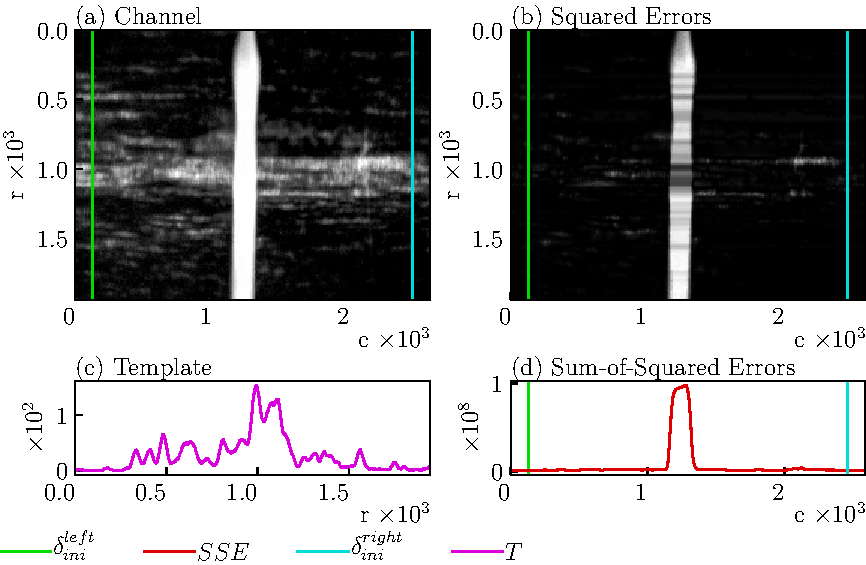
\includegraphics[width=\linewidth]{template_matching.pdf} 
\caption{Template matching with $\delta^{left}_{ini}=C-\delta^{right}_{ini}=130$.}
\label{fig: template_matching}
\end{figure} 

\begin{figure}[!h]
\centering
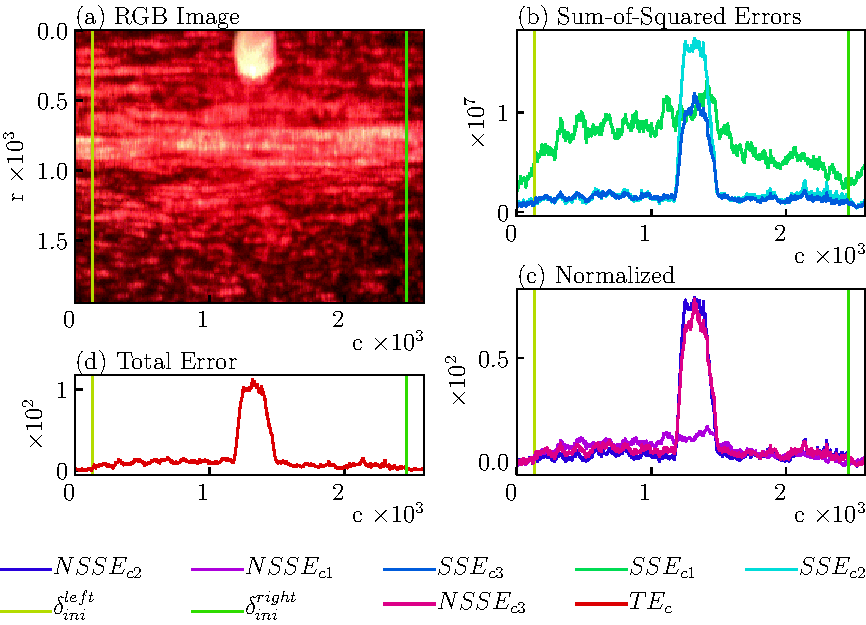
\includegraphics[width=\linewidth]{normalized.pdf} 
\caption{Total Error as euclidean distance of normalized sum-of-squared errors.}
\label{fig: normalized}
\end{figure}

\begin{figure}[!h]
\centering
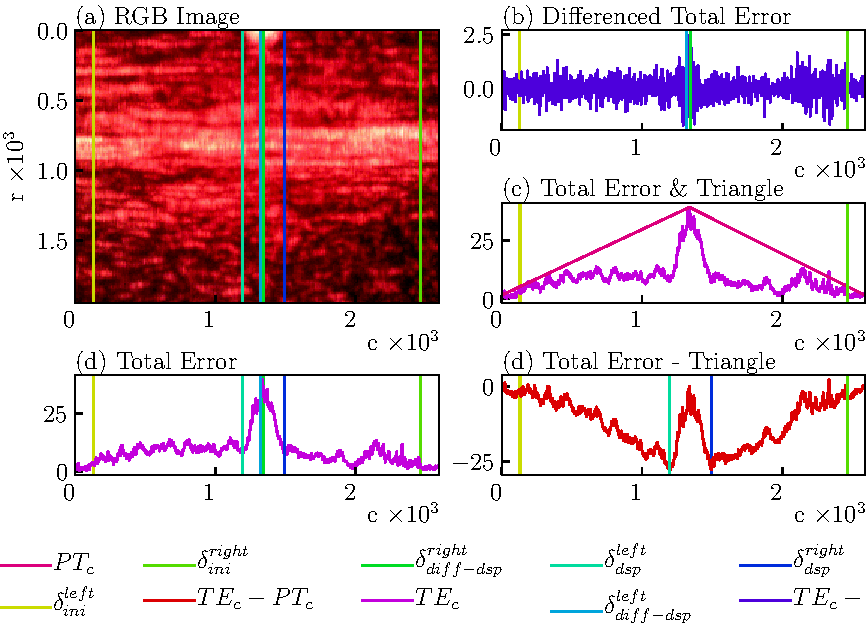
\includegraphics[width=\linewidth]{triangle.pdf} 
\caption{Triangle based segmentation versus differencing.}
\label{fig: triangle}
\end{figure}

\begin{figure}[!ht]
\centering
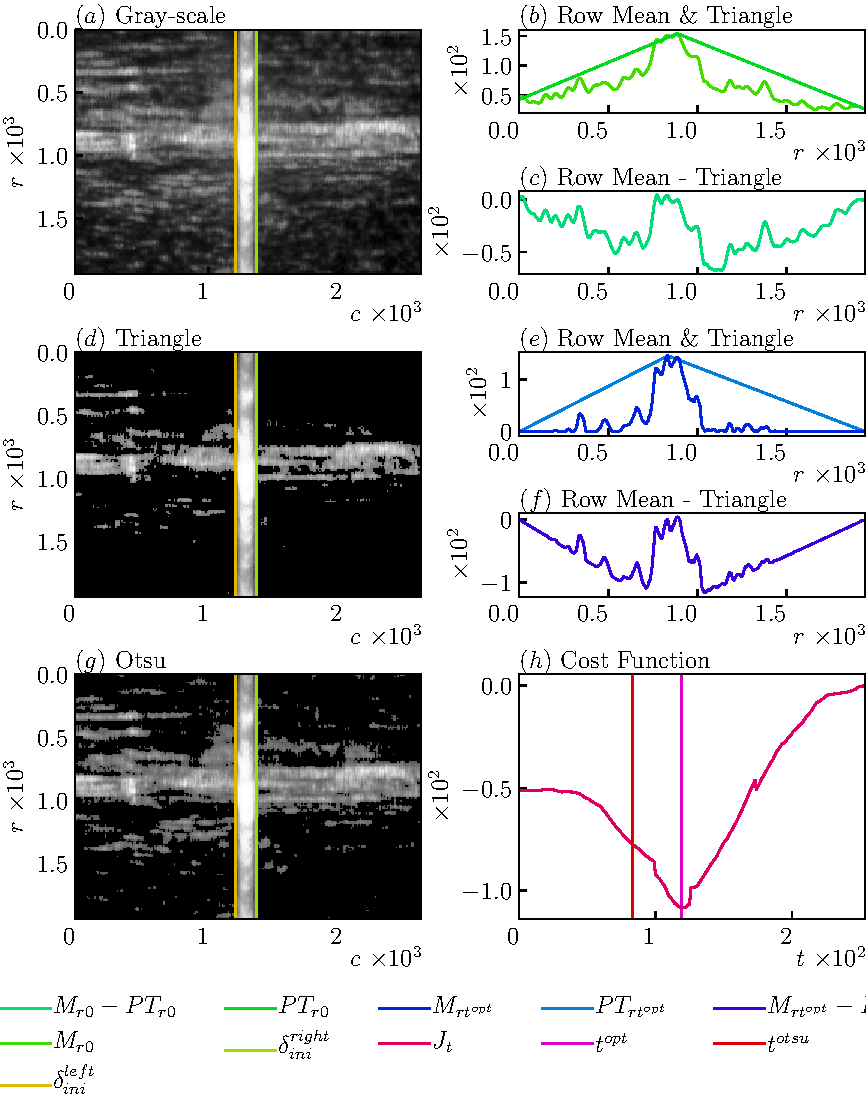
\includegraphics[width=\linewidth]{thresholding.pdf} 
\caption{Triangle based thresholding versus Otsu's method.}
\label{fig: thresholding}
\end{figure}

Figure \ref{fig: edge_segmentation}(abc) shows the edge segment found for the original as well as the thresholded gray scale image and the resulting row mean.
\begin{figure}[!ht]
\centering
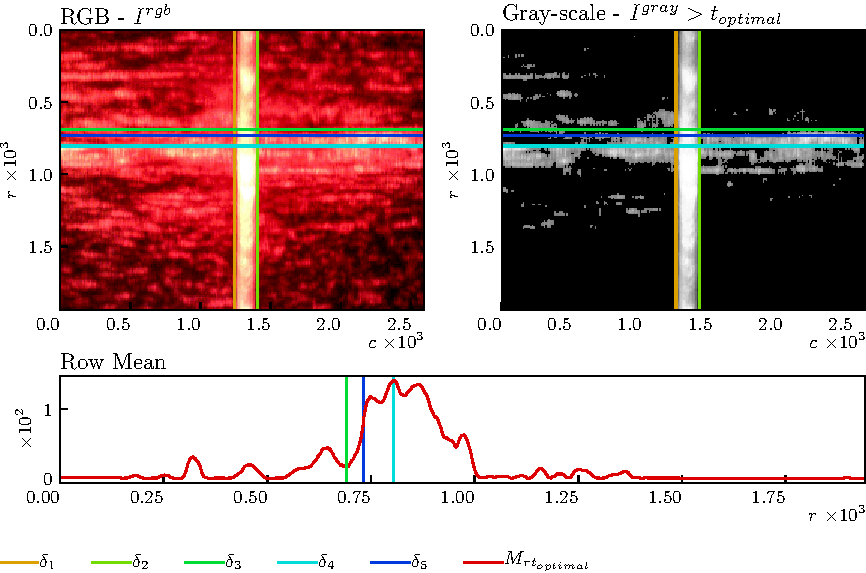
\includegraphics[width=\linewidth]{edge_segmentation.pdf} 
\caption{Edge segmentation of the laser line on the print bed.}
\label{fig: edge_segmentation}
\end{figure}


\begin{figure}[!ht]
\centering
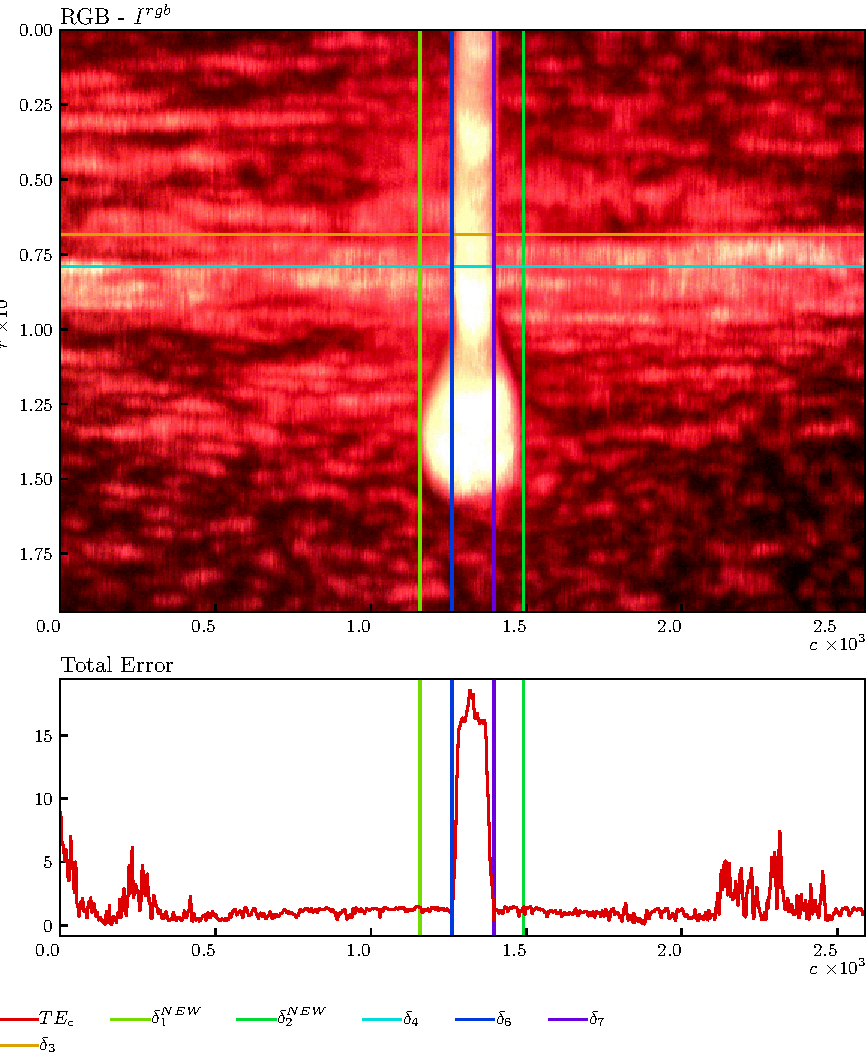
\includegraphics[width=\linewidth]{width_extraction.pdf} 
\caption{Width extraction at the position of the laser line edge.}
\label{fig: width_extraction}
\end{figure}

\begin{figure}[!ht]
\centering
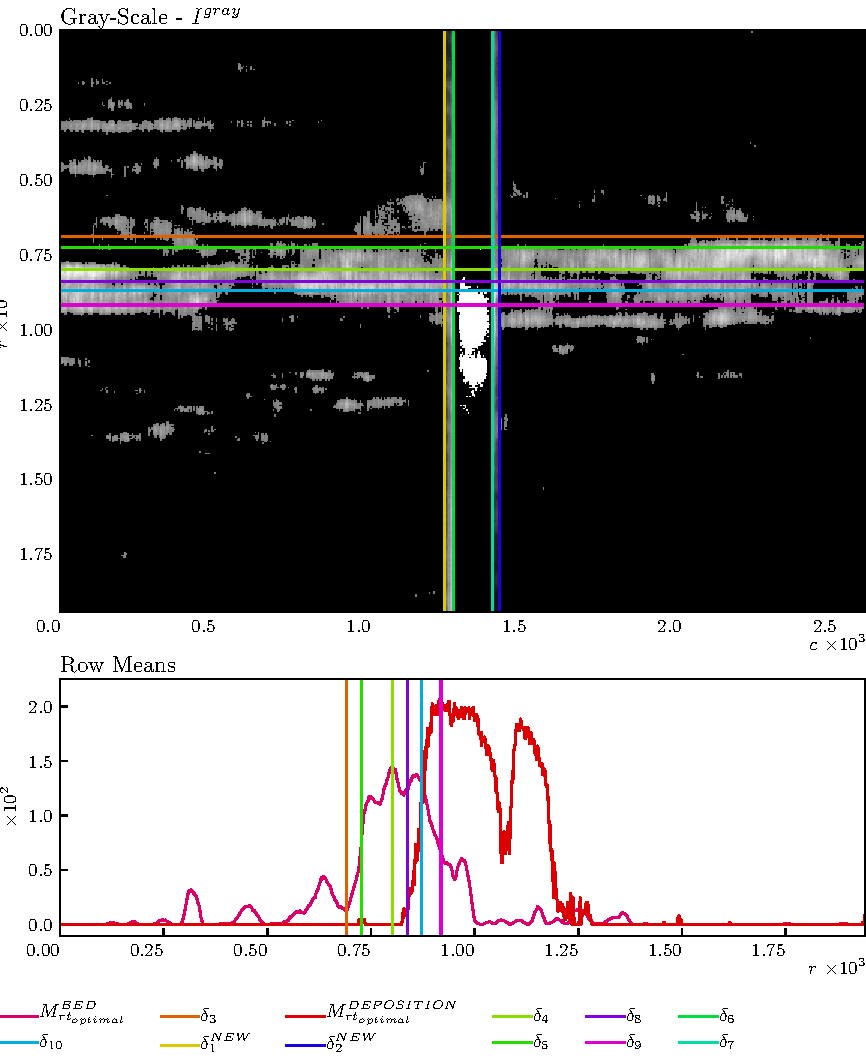
\includegraphics[width=\linewidth]{height_extraction.pdf} 
\caption{Height extraction.}
\label{fig: height_extraction}
\end{figure}

\end{document}